\chapter{Introduction}
\label{chap:introduction}

Image Anomaly detection (IAD) as a form of quality control is a widely popular practice in modern manufacturing processes. In the last 74 years, the steel production worldwide, 
has increased by more than ninefold \cite{worldsteel}, due to innovation and a growing usage of metal in modern applications. 
With these developments, there came a high need for quality 
assurance alongside raised standards and requirements. These strict conditions serve, among other things 
to avoid product failure in situations that could cause fatal consequences. Quality control in form of anomaly detection often 
starts at the individual parts manufactured for a single purpose, which demands a large effort and lots of resources due to factors like 
the above-mentioned increasing production rate. 
In earlier days this meant procedures like manual stochastic quality checks of produced parts, a practice that in its nature cannot give 
complete certainty, is very labor-intensive and therefore, comes at a high price point for the manufacturers. Later, with the rise of computers and sophisticated computer vision methods 
this process of quality control became increasingly automated, with methods like IAD ensuring a more efficient quality control procedure. With time, these developments, 
alongside a constant striving of industries towards even higher reliability, and later the recent developments in artificial intelligence brought forth IAD as the 
well researched research field it is today.\newline 
IAD, in our context, is a subcategory of general anomaly detection 
and aims at distinguishing images of a category that conform to some chosen norm from anomalous images of the same category that do not. 
An example would be creating a classifier that is given the image of a screw and can detect whether it conforms to our expectations, 
which in a manufacturing setting likely means to meet the company's quality standards(Fig. \ref{fig:introscrew}).

\begin{figure}[htbp]
    \captionsetup[subfigure]{justification=centering}
    \centering
    \begin{subfigure}[b]{0.28\textwidth}
        \centering
        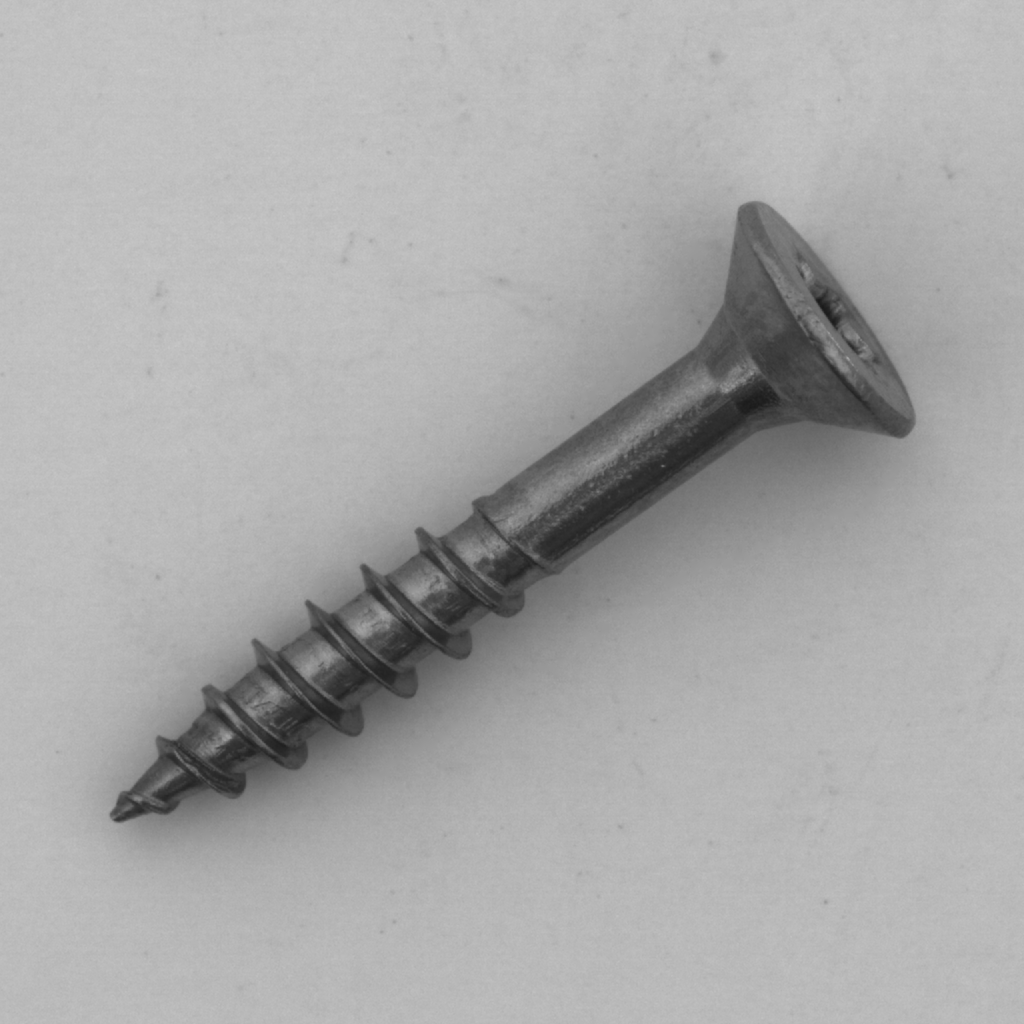
\includegraphics[width=\textwidth]{figures/introductionanomalies/033.png}
        %\caption*{original Image}

    \end{subfigure}
    \hspace{0.05\textwidth} % Add space between subfigures
    \begin{subfigure}[b]{0.28\textwidth}
        \centering
        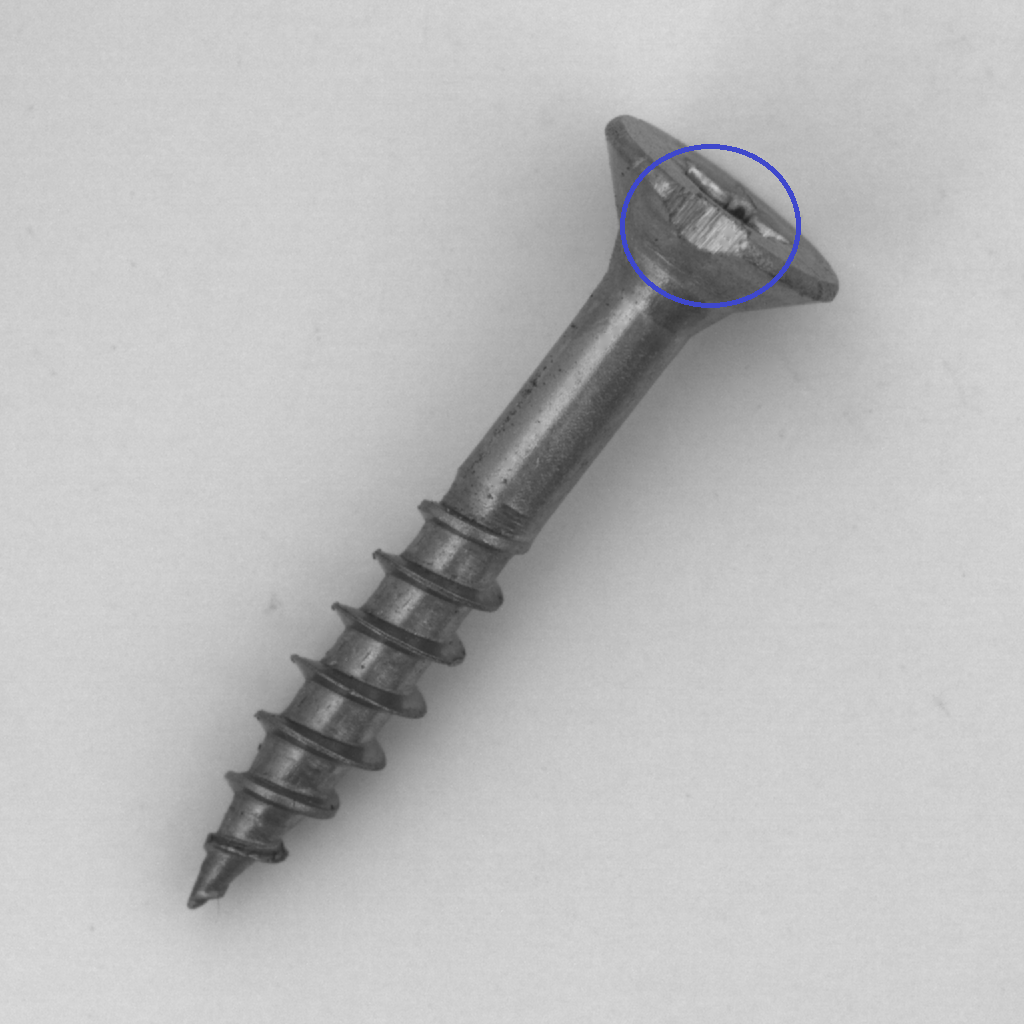
\includegraphics[width=\textwidth]{figures/introductionanomalies/manifrontcopy.png}
        %\caption*{Mask}

    \end{subfigure}
    \hspace{0.05\textwidth} % Add space between subfigures
    \begin{subfigure}[b]{0.28\textwidth}
        \centering
        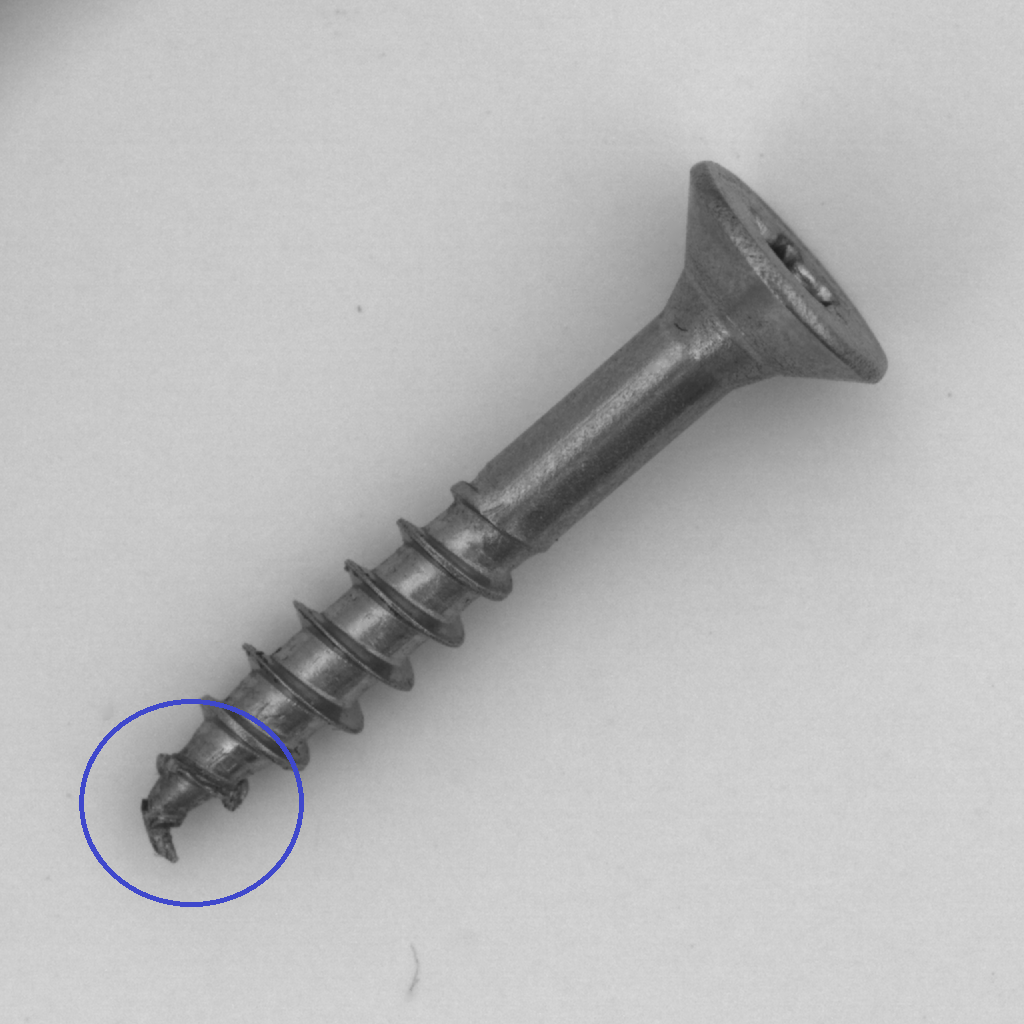
\includegraphics[width=\textwidth]{figures/introductionanomalies/realfrontnow.png}
        %\caption*{Discriminator Predictions}

    \end{subfigure}
    \caption{Instance images of a screw from \cite{MVTEC_Bergmann_2021} to showcase anomalous objects in manufacturing settings. The images include a regular screw, a screw with a chipped head and a screw with a bent tip.}
    \label{fig:introscrew}
\end{figure}

With IAD, being a very recent and popular field, there are various deep learning apporaches that have established themselves over 
the last couple of years. The best performing ones have generally been unsupervised learning approaches. This stems from the fact, that 
in any manufacturing setting, there usually exist far less anomalous parts than regular ones, which creates a significant data imbalance. 
Moreover, it can pose as difficult to actually obtain a large number of data points and great variance, since it is a lot of work to 
coordinate with adequate manufacturing facilities and implement the necessary infrastructure to take pictures. This problem is supported 
by the fact that there are little well established datasets being used for modern IAD research. There are still some credible and widely used 
datasets, amongst them the MVTecAD \cite{MVTEC_Bergmann_2021} dataset acting as a gold standard. The dataset will be discussed in greater detail 
in the background chapter. Regarding the kind of unsupervised anomaly detection methods, there is again a great variety of approaches that follow a 
distinct strategy of differentiating between the classes. Still most of them can be categorized with two classes: representation- 
or reconstruction-based methods. While representation approaches aim at creating a feature representation to then 
compare the features of new input images, reconstruction-based ones try to learn how to recreate the part shown in the image as an anomaly 
free object, and then comparing the constructed product to the original input. Both workflows are visualized in figure \ref{fig:vizofrecrepbased}, which showcases 
the individual steps of the respective methods as described. It is to be said that both approaches offer high quality predictions, yet 
feature representation methods have more frequently shown in latest research to achieve state of the art results \cite{liu2024deep}. % \cite{Xie_2024benchmarking}.
\newline
The current state of IAD generally consists of very high performing classifiers. Here it is important to differentiate between the  
applications of those classifiers. There is anomaly detection in form of image classification, which was already mentioned. 
Furthermore, there is anomaly localization, referring to the process of image segmentation to point out the specific regions in which 
the detected anomaly occurs. Lastly besides the applications, one can also categorize kinds of anomalies. The most researched anomaly types 
are so called structural anomalies, which can be described as superficial damages of the parts material or shape, i.e. a strongly 
bent screw or one that is broken in the middle. Yet recently there has been a new dataset from the creates of MVTecAD that covers logical 
anomalies, namely the MVTecAD LOCO \cite{LOCODentsAndScratchesBergmann2022} dataset. Logical anomalies denote ones that violate an abstract 
set of rules. More concretely this can mean instances like a metal part with an irregular number of holes, or a label missing. Whereas 
state of the art approaches produce performance metrics of up to $99.6 \% $ on classifying structural anomalies, they 
strongly diverge in anomaly localization performance. Moreso does the performance plummet when approaching to classify and localize logical 
anomalies. Additionally models often show inconsistencies between individual subtypes of structural and logical anomalies, especially during 
localization. Another important consideration is, that most anomaly detection approaches have distinct weaknesses, which worsen most 
of their performances in certain situations. These inconsistencies and performance gaps demonstrate that IAD as such is not yet solved and still has a need for improved 
robustness and generalizability. This need also holds true due to logical anomalies making up an important new domain of automated 
quality control, as more complex parts could be tested for requirements. Moreover, the showcasing of performance inconsistencies between 
structural and logical anomalies indicate the latter being of a different problem domain. Achieving better translation between those 
settings could serve as a basis for tackling other problems in this field that may arise in future settings.


\section{Contributions}
\label{sec:contributions}
This research provides multiple contributions to the field of image anomaly detection, in an effort to provide a structured overview of current IAD research and 
further push the progress of robust anomaly localization. 

\begin{enumerate}
  \item To address the problems mentioned at the end of the last section, we attempt 
  to build a feature level ensemble network, combining various feature representations with the goal to improve 
  general performance alongside robustness in logical anomaly localization and detection. This ensemble network is then tested on 
  the MVTecAD LOCO dataset to observe its performance regarding both anomaly types.
  \item Furthermore, an extensive study on the performance of a diverse selection of IAD methods on the MVTecAD LOCO dataset is performed. 
  This serves to highlight the current state of anomaly detection with respect to logical problems, and also investigate the application potential of 
  those approaches a form of transfer learning setting.
  \item Second to last, we introduce a new category to the MVTecAD LOCO dataset to further increase the diversity of this dataset and strengthen the focus 
  of this thesis on metal manufactured parts. Many datasets either use synthetic data or images in a very clinical setting, therefore this 
  attempt for variance is also a step towards IAD on more realistic datasets.
  \item Finally, the mentioned network and experiments are also streamlined into an easy to use pipeline 
  to be used for future experiments in that area.
\end{enumerate}

The contributions mentioned firstly benefit faster research entry and an accelerated experimentation process, with an intuitive setup, 
as well as potential industrial applications. 
Furthermore they give more insight into the capabilities of existing methods in an industrial setting and thus also provide a more 
diverse and practical setting than the prior categories in the MVTecAD \cite{LOCODentsAndScratchesBergmann2022} dataset. The same methods are also tested on their limitations 
regarding logical anomalies which was earlier made out to be a relevant aspect of anomaly detection in current manufacturing quality control 
settings. Lastly through the use of a robust ensemble approach for potentially heterogeneous classifiers, this opens up possibilities for expanding 
the range of application of state of the art IAD methods to other domains with robust performance and may also produce more usable results in real 
world IAD settings. The presented network can also be used as a foundation for future experiments in 
various directions. Possible outlooks based on this kind of multi-feature representation ensembles are discussed in section \ref{sec:finaloutlook}.
\newline
\newline

In this work we will firstly discuss relevant background knowledge to get a grasp on the latest important IAD research, as well as fundamental principles that are relevant to the ensemble 
approach presented here. Section \ref{sec:IADcategs} and section \ref{sec:IADmethods} give a broad overview of state of the art IAD approaches as well as intuitive knowledge on how to 
view them. Afterwards sections \ref{sec:metrics} and \ref{sec:datasets} offer in insight into the testing and evaluation environments of this context. Lastly section \ref{sec:ensembles} and 
section \ref{sec:modelcalibration} are focused on background knowledge to common approaches regarding the ensemble model talked about before.\newline
The third chapter presents the novel dataset category introduced in this paper.
In chapter \ref{chap:method} we present the concrete implementation of this works contributions, starting with section \ref{sec:lcocsurveymethods} dealing with the survey on logical anomalies. 
Section \ref{sec:ourensemblenetwork} concerns the realization of this ensemble approach.
\newline 
Chapters \ref{chap:results} and \ref{chap:conclusion} afterwards deal with an in depth analysis of our findings as well as an outlook on how to interpret these results and what future research 
in this topic may look like.






